\documentclass[11pt,letterpaper]{article}
\usepackage{style}

%% ------- INICIA DOCUMENTO ------
\begin{document}
\begin{titlepage}
\begin{center}
\begin{LARGE}
INSTITUTO POLITÉCNICO NACIONAL\\
\vspace*{0.15in}
ESCUELA SUPERIOR DE CÓMPUTO\\
\end{LARGE}
\vspace*{1.0in}
\begin{Large}
%% NOMBRE DE LA PRÁCTICA O EXAMEN
\textbf{TÉCNICAS DE CRUZA 1} \\  
\end{Large}
\vspace*{0.2in}
\begin{large}
\textit{Práctica 6}\\
\end{large}
\vspace*{1.0in}
\begin{large}
%% INTEGRANTES	
Dominguez de la Rosa Bryan\\
\vspace*{2.0in}
GRUPO 3CM5\\
\vspace*{0.2in}
Profesor: Morales Güitron Sandra Luz\\
\vspace*{1.5in}
\today
\vspace*{0.3in}
\end{large}
\rule{150mm}{0.1mm}\\

\end{center}
\end{titlepage}

%% --------- COMIENZA EL DESARROLLO DEL DOCUMENTO --------

\section*{Introducción}


\section*{Contenido}
Para la implementación del algoritmo de ruleta, implementé 4 arreglos de bits para controlar las distintas etapas que se realizan en el algoritmo:
\begin{itemize}
	\item Población inicial.
	\item Población de individuos seleccionados por ruleta.
	\item Población después de cruza.
	\item Población después de mutación.
\end{itemize}

En la primer etapa, se llena aleatoriamente el arreglo de población inicial con series de 5 bits. Una vez que se tiene la primer población, se ejecuta el algoritmo de ruleta, de la siguiente forma:

\begin{enumerate}
	\item Se genera un número aleatorio entre 0 y el valor de la aptitud total de la población inicial.
	\item Se genera un ciclo en el que en se acumulará la aptitud total de cada individuo de la población.
	\item El ciclo se detiene cuando la suma acumulada supere el valor aleatorio generado.
	\item El padre seleccionado será el individuo que genere que se sobrepase el valor aleatorio generado. 
\end{enumerate}

\begin{figure}[H]
	\centering
	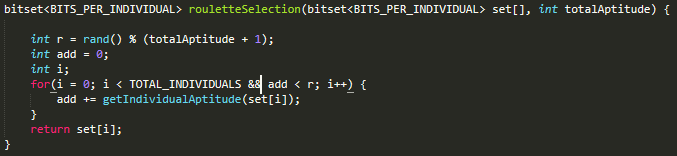
\includegraphics[scale = 1]{images/ruleta}
	\caption{Algoritmo genético de selección de ruleta}
\end{figure}

Una vez teniendo la población de selección de padres, se realiza una cruza de individuos de la siguiente manera:

\begin{enumerate}
	\item Se utilizan 2 individuos de la población de padres.
	\item Se define un punto de cruza estático para todas las generaciones.
	\item Se cruzan los individuos.
	\item Se retorna el individuo resultante.
\end{enumerate}

\begin{figure}[H]
	\centering
	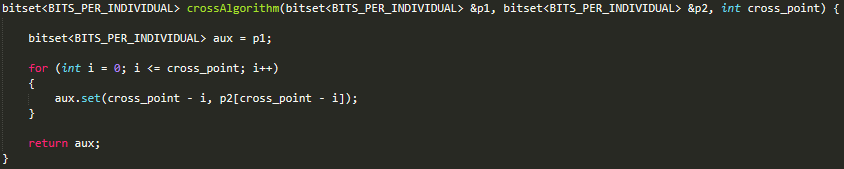
\includegraphics[scale = .8]{images/cruza}
	\caption{Algoritmo de cruza de individuos}
\end{figure}

Al obtener la población de individuos después de la cruza se necesita realizar una mutación. En este caso se generó una mutación del 10\% de la población. Nuestra población total es de 32 elementos, entonces la cantidad de individuos a redondear es 3.2, redondeado como 3.\\

La mutación se realiza de la siguiente forma:
\begin{enumerate}
	\item El algoritmo se realizará 3 veces.
	\item La mutación buscará mejorar al individuo, por lo tanto, se buscará cambiar un bit 0 por un bit 1.
	\item Debido a que se requiere buscar un 0 en el individuo a mutar, y es posible que el individuo no tenga bits 0, se define un número máximo de iteraciones para evitar que el programa se cicle.
	\item Cuando se encuentre un bit 0, se cambia por un bit 1.
\end{enumerate}

\begin{figure}[H]
	\centering
	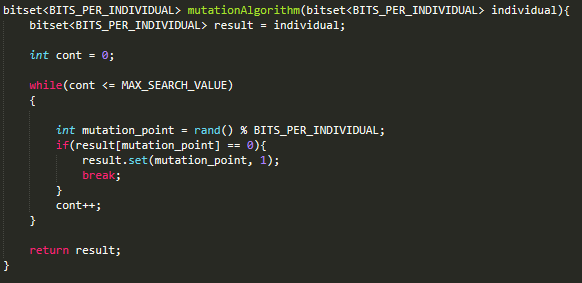
\includegraphics[scale = 1]{images/mutacion}
	\caption{Algoritmo de mutación de individuos}
\end{figure}

Una vez que se tenga la población mutada, se establece ésta como población inicial, para realizar el algoritmo de ruleta en la siguiente generación.\\

Al obtener la población final de una generación, se obtiene la aptitud del individuo de menor valor, la aptitud del individuo de mayor valor y el promedio de aptitud de cada generación.\\

Ejemplo con 5 generaciones:
\begin{figure}[H]
	\centering
	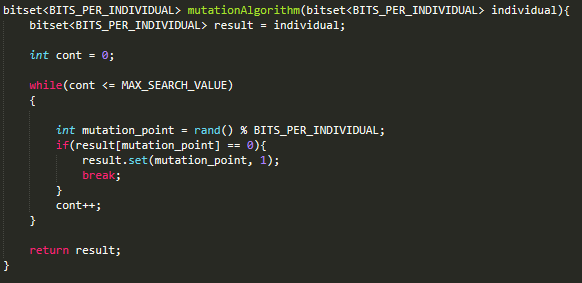
\includegraphics[scale = 1]{images/mutacion}
	\caption{Resultado de 5 generaciones}
\end{figure}

Ejemplo con 10 generaciones:
\begin{figure}[H]
	\centering
	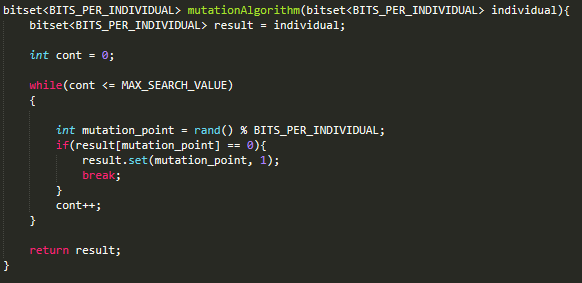
\includegraphics[scale = 1]{images/mutacion}
	\caption{Resultado de 10 generaciones}
\end{figure}

Ejemplo con 15 generaciones:
\begin{figure}[H]
	\centering
	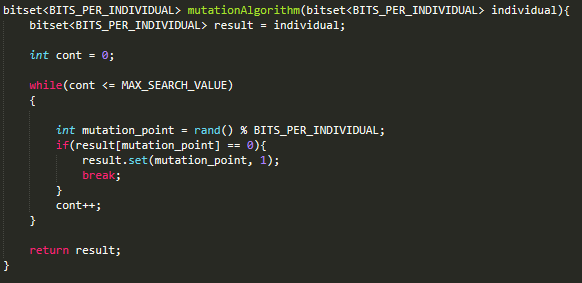
\includegraphics[scale = 1]{images/mutacion}
	\caption{Resultado de 10 generaciones}
\end{figure}


\section*{Conclusión}


\end{document}


